% Dit werk is gelicenseerd onder de licentie Creative Commons Naamsvermelding-GelijkDelen 4.0 Internationaal. Ga naar http://creativecommons.org/licenses/by-sa/4.0/ om een kopie van de licentie te kunnen lezen.
\documentclass[t]{beamer}

%%%%%%%%%%%%%%%%%%%%%%%%%%%%%%
% Packages
%%%%%%%%%%%%%%%%%%%%%%%%%%%%%%

\usepackage[dutch]{babel}               % Voor nederlandstalige hyphenatie (woordsplitsing)
\uselanguage{dutch}
\languagepath{dutch}
\usepackage{url}                        % Om url's te verwerken
\usepackage{graphicx,subfigure}         % Om figuren te kunnen verwerken
\usepackage[utf8]{inputenc}             % Om niet ascii karakters rechtstreeks te kunnen typen
\usepackage{multicol}
\usepackage[absolute,overlay]{textpos}

%%%%%%%%%%%%%%%%%%%%%%%%%%%%%%
% Layout
%%%%%%%%%%%%%%%%%%%%%%%%%%%%%%
\usetheme{Frankfurt}
\usefonttheme[onlymath]{serif}
\setbeamertemplate{footline}[page number]
\AtBeginSection[]
{
  \begin{frame}
    \frametitle{Inhoud}
    \tableofcontents[currentsection]
  \end{frame}
}

\setbeamertemplate{navigation symbols}{}

%%%%%%%%%%%%%%%%%%%%%%%%%%%%%%
% Title
%%%%%%%%%%%%%%%%%%%%%%%%%%%%%%
\title{Inleiding tot Inkscape}
\author{Brecht Baeten\inst{1}}
\institute{
	\inst{1}%
  		e-mail: brecht.baeten@gmail.com
}
\date{\today}
%%%%%%%%%%%%%%%%%%%%%%%%%%%%%%
% Omgevingen
%%%%%%%%%%%%%%%%%%%%%%%%%%%%%%

\begin{document}
	\frame{\titlepage}
%%%%%%%%%%%%%%%%%%%%%%%%%%%%%%%%%%%%%%%%%%%%%%%%%%%%%%%%%%%%%%%%%%%%%%%%%%%%%%%%
	\section{Inleiding}
%%%%%%%%%%%%%%%%%%%%%%%%%%%%%%%%%%%%%%%%%%%%%%%%%%%%%%%%%%%%%%%%%%%%%%%%%%%%%%%%
	\begin{frame}
		\frametitle{Voorbeelden}
		%\center
    	%\includegraphics[height=0.7\textheight{fig/inleiding/building_neighbourhood_cfd}\\
	\end{frame}
%%%%%%%%%%%%%%%%%%%%%%%%%%%%%%%%%%%%%%%%%%%%%%%%%%%%%%%%%%%%%%%%%%%%%%%%%%%%%%%%
	\section{Vector graphics}
%%%%%%%%%%%%%%%%%%%%%%%%%%%%%%%%%%%%%%%%%%%%%%%%%%%%%%%%%%%%%%%%%%%%%%%%%%%%%%%%
	\begin{frame}
		\frametitle{Bitmap vs. Vector}
		\vspace{0.5cm}
		\begin{columns}
			\begin{column}[T]{0.5\textwidth}
				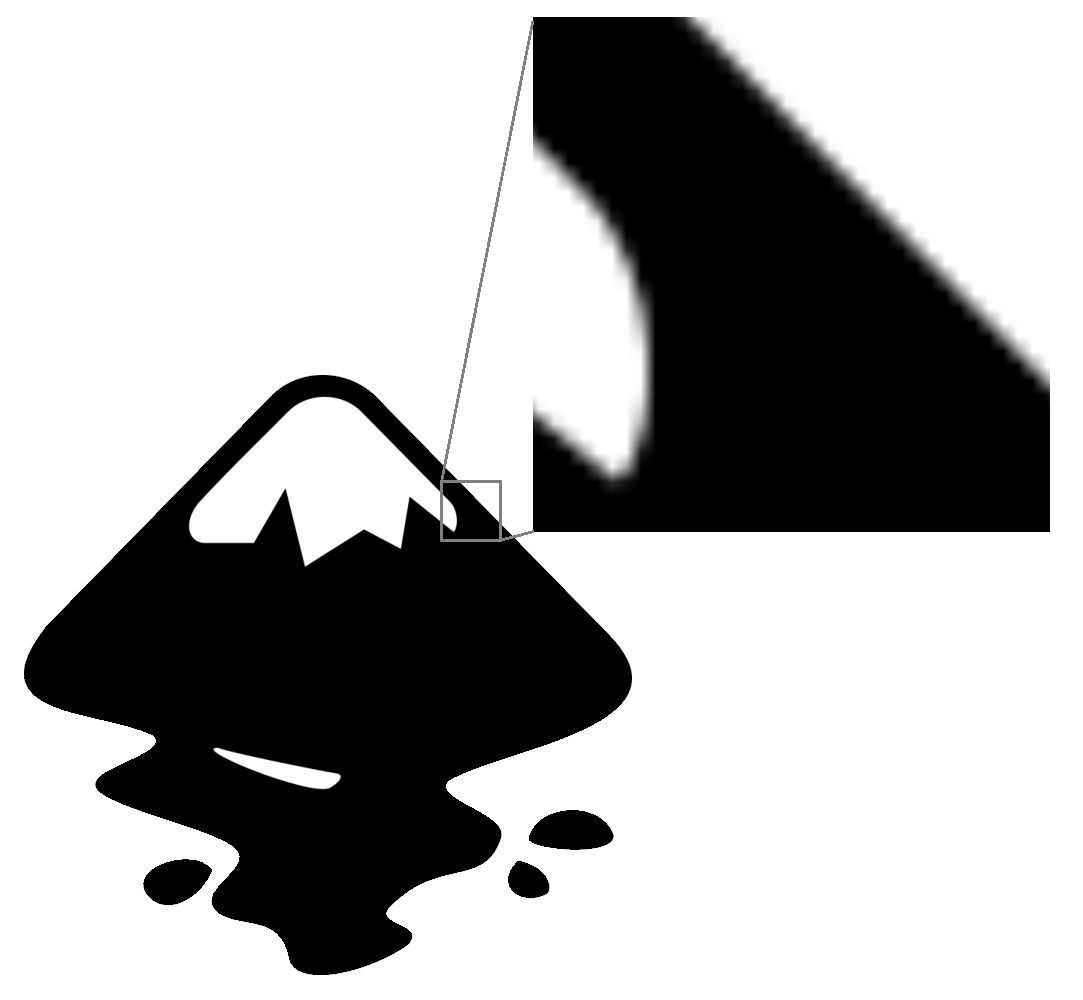
\includegraphics[width=\textwidth]{fig/logo_zoom_png}
				\vspace{0.5cm}
				.bmp, .png, .jpg,...
			\end{column}
			\begin{column}[T]{0.5\textwidth}
				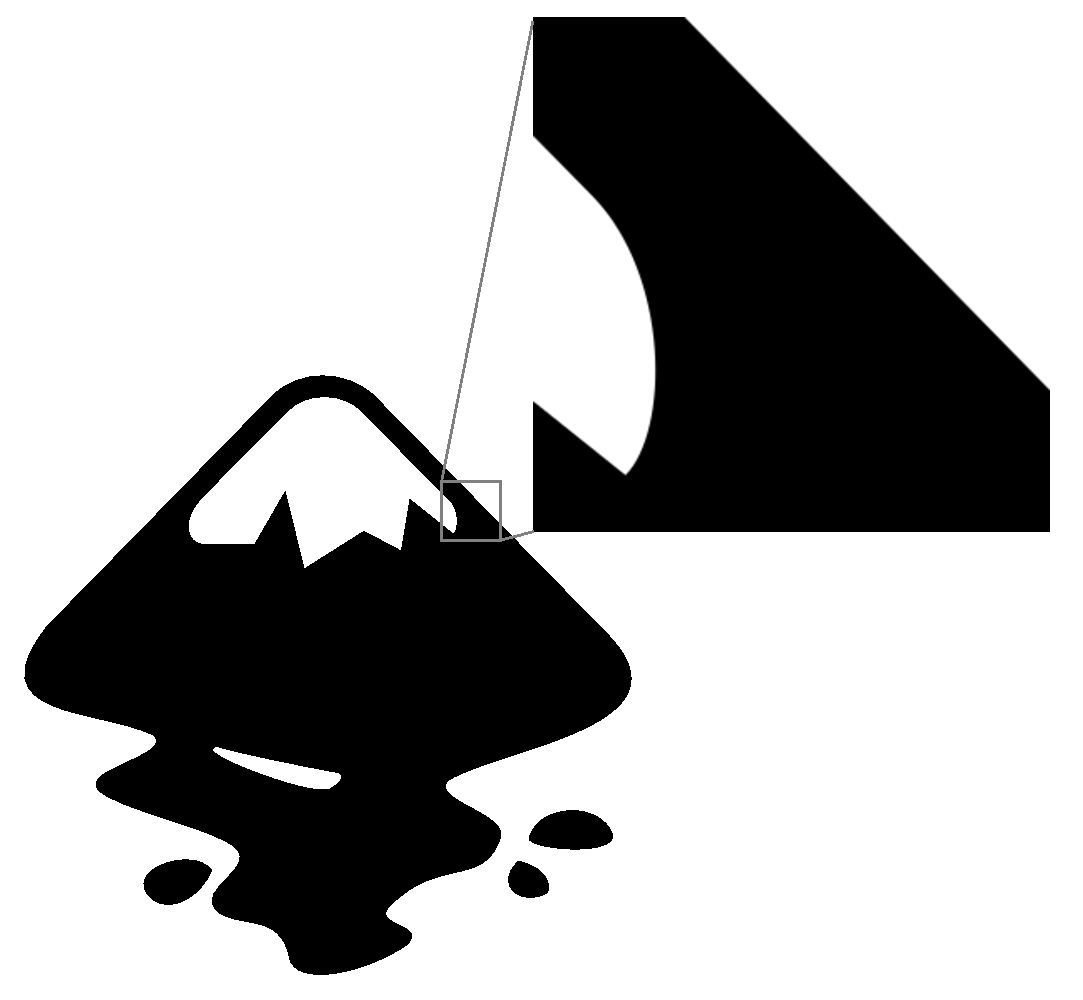
\includegraphics[width=\textwidth]{fig/logo_zoom_pdf}
				\vspace{0.5cm}
				.svg, .eps, .cdr, .ai, .pdf,...
			\end{column}
		\end{columns}
	\end{frame}
%%%%%%%%%%%%%%%%%%%%%%%%%%%%%%%%%%%%%%%%%%%%%%%%%%%%%%%%%%%%%%%%%%%%%%%%%%%%%%%%
	\begin{frame}
		\frametitle{Scalable Vector Graphics}
		\begin{itemize}
			\item .svg
			\item W3C norm (zoals html, css, xml,...)
			\item "leesbare" bestanden
			\item "definitie" van de tekening
		\end{itemize}
		\vspace{0.5cm}
		\begin{center}
			\hfill 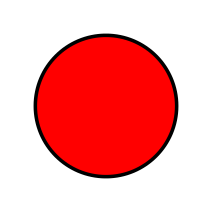
\includegraphics[width=0.2\textwidth]{fig/simpele_tekening}\\
			\vspace{-0.2cm}
			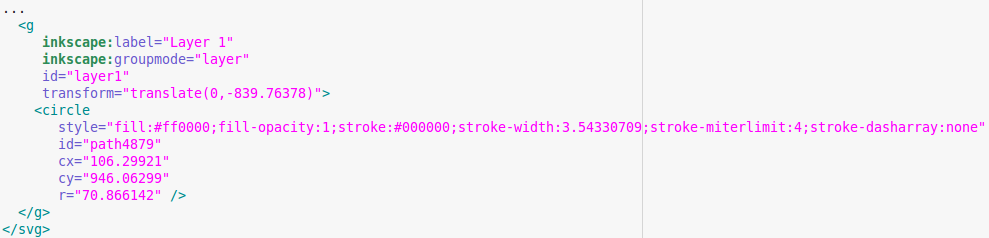
\includegraphics[width=\textwidth]{fig/simpele_tekening_bron.png}
		\end{center}	
	\end{frame}
%%%%%%%%%%%%%%%%%%%%%%%%%%%%%%%%%%%%%%%%%%%%%%%%%%%%%%%%%%%%%%%%%%%%%%%%%%%%%%%%
	\section{Inkscape}
%%%%%%%%%%%%%%%%%%%%%%%%%%%%%%%%%%%%%%%%%%%%%%%%%%%%%%%%%%%%%%%%%%%%%%%%%%%%%%%%
	\begin{frame}
		\frametitle{Werkbalken}
		\begin{center}
			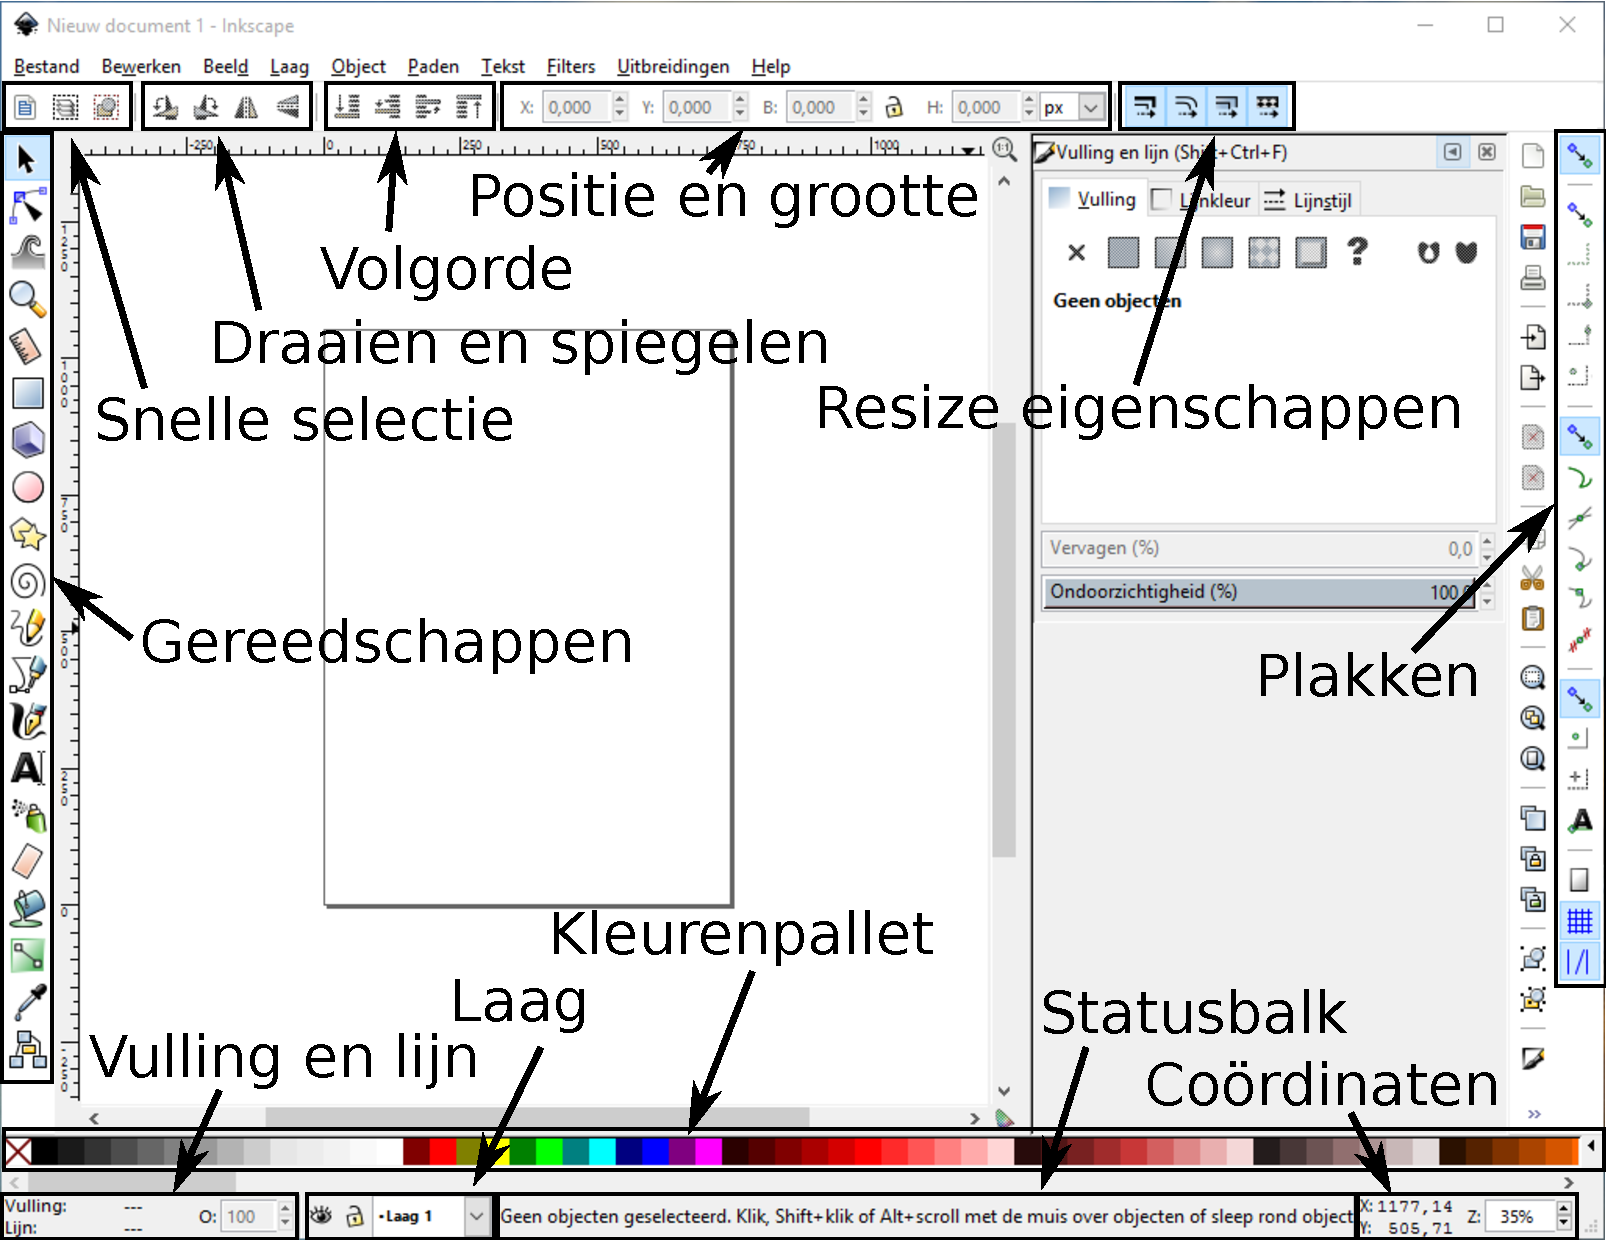
\includegraphics[height=0.85\textheight]{fig/inkscape_werkbalken}\\
		\end{center}	
	\end{frame}
%%%%%%%%%%%%%%%%%%%%%%%%%%%%%%%%%%%%%%%%%%%%%%%%%%%%%%%%%%%%%%%%%%%%%%%%%%%%%%%%
	\section{Objecten en Paden}
%%%%%%%%%%%%%%%%%%%%%%%%%%%%%%%%%%%%%%%%%%%%%%%%%%%%%%%%%%%%%%%%%%%%%%%%%%%%%%%%
	\begin{frame}
		\frametitle{Objecten}
		\begin{columns}
			\begin{column}[T]{0.5\textwidth}
				\begin{itemize}
					\item Rechthoek
					\item 3D doos
					\item Cirkel
					\item Veelhoek / ster
					\item Spiraal
					\item Tekst
				\end{itemize}
			\end{column}
			\begin{column}[T]{0.5\textwidth}
				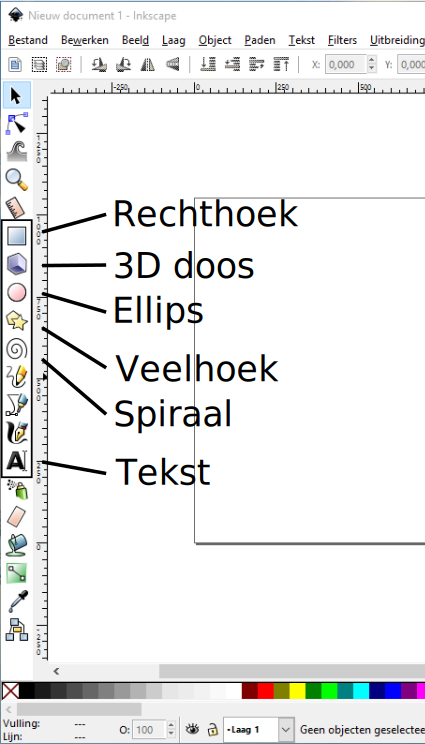
\includegraphics[height=0.8\textheight]{fig/inkscape_objecten}
			\end{column}
		\end{columns}
	\end{frame}
%%%%%%%%%%%%%%%%%%%%%%%%%%%%%%%%%%%%%%%%%%%%%%%%%%%%%%%%%%%%%%%%%%%%%%%%%%%%%%%%
	\begin{frame}
		\frametitle{Objecten en kleuren}
		\only<1>{
			\begin{center}
				
\includegraphics[height=0.8\textheight]{fig/objecten_en_kleuren}
			\end{center}
		}
		\only<2>{
			\begin{itemize}
				\item Vulling en lijn pallet openen via \emph{Object $>$ Vulling en lijn...}\\
				 of \textbf{Ctrl} + \textbf{Shift} + F\\
				 of dubbelklikken op vulling en lijn detail (links onderaan)
				\item Vulling, Lijnkleur, Lijnstijl
			\end{itemize}
			
			\vspace{0.5cm}
			\textbf{Extra's:}
			\begin{itemize}
				\item kleurenpallet klik = vulling kleur
				\item \textbf{Shift} + kleurenpallet klik  = rand kleur
			\end{itemize}
		}
	\end{frame}
%%%%%%%%%%%%%%%%%%%%%%%%%%%%%%%%%%%%%%%%%%%%%%%%%%%%%%%%%%%%%%%%%%%%%%%%%%%%%%%%
	\begin{frame}
		\frametitle{Objecten draaien en transformeren}
		\only<1>{
			\begin{center}
				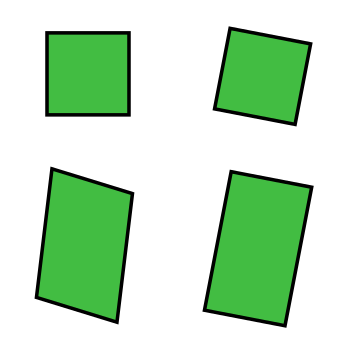
\includegraphics[height=0.8\textheight]{fig/objecten_draaien_en_transformeren}
			\end{center}
		}
		\only<2>{
			\begin{center}
				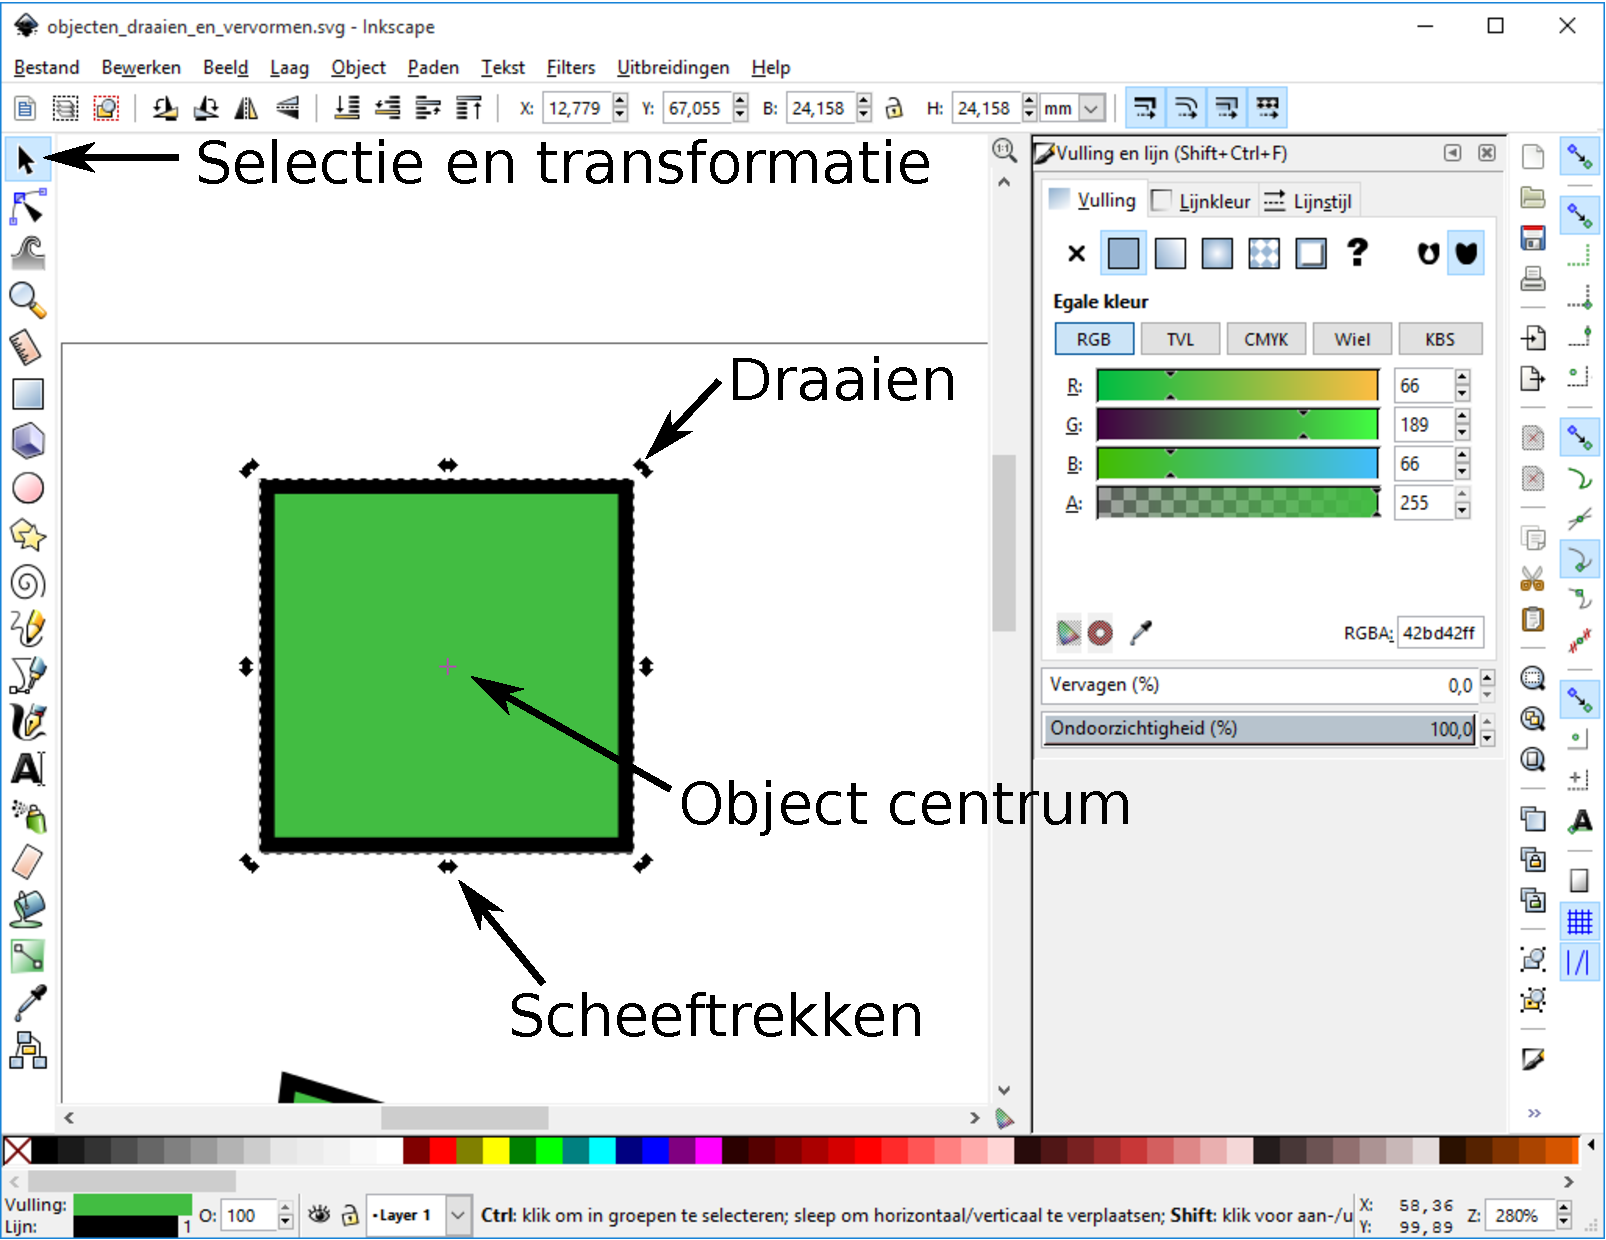
\includegraphics[height=0.8\textheight]{fig/inkscape_objecten_draaien_en_transformeren}
			\end{center}
		}
		\only<3>{
			Ieder object heeft zijn eigen specifieke vervormings eigenschappen, beschikbaar via het object gereedschap
			
			\vspace{0.5cm}
			\textbf{Extra's:}
			\begin{itemize}
				\item \textbf{Ctrl} + vervormen = behoud van aspect ratio
				\item \textbf{Shift} + vervormen = schalen rond middelpunt
				\item \textbf{Ctrl} + \textbf{Shift} + vervormen = combinatie van bovenstaande
				\item \textbf{Ctrl} + draaien = draaien met stappen van 15$^\circ$
				\item \textbf{Ctrl} + slepen = horizontaal of verticaal slepen
				\item slepen + \textbf{spatie} = object dupliceren en plaatsen
			\end{itemize}
		}
		
	\end{frame}
%%%%%%%%%%%%%%%%%%%%%%%%%%%%%%%%%%%%%%%%%%%%%%%%%%%%%%%%%%%%%%%%%%%%%%%%%%%%%%%%
	\begin{frame}
		\frametitle{Paden}
		
	\end{frame}
%%%%%%%%%%%%%%%%%%%%%%%%%%%%%%%%%%%%%%%%%%%%%%%%%%%%%%%%%%%%%%%%%%%%%%%%%%%%%%%%
	\section{Document eigenschappen}
%%%%%%%%%%%%%%%%%%%%%%%%%%%%%%%%%%%%%%%%%%%%%%%%%%%%%%%%%%%%%%%%%%%%%%%%%%%%%%%%



%%%%%%%%%%%%%%%%%%%%%%%%%%%%%%%%%%%%%%%%%%%%%%%%%%%%%%%%%%%%%%%%%%%%%%%%%%%%%%%%	
	\section{Templates}
%%%%%%%%%%%%%%%%%%%%%%%%%%%%%%%%%%%%%%%%%%%%%%%%%%%%%%%%%%%%%%%%%%%%%%%%%%%%%%%%



%%%%%%%%%%%%%%%%%%%%%%%%%%%%%%%%%%%%%%%%%%%%%%%%%%%%%%%%%%%%%%%%%%%%%%%%%%%%%%%%		
	\section{Afbeeldingen importeren}
%%%%%%%%%%%%%%%%%%%%%%%%%%%%%%%%%%%%%%%%%%%%%%%%%%%%%%%%%%%%%%%%%%%%%%%%%%%%%%%%	



%%%%%%%%%%%%%%%%%%%%%%%%%%%%%%%%%%%%%%%%%%%%%%%%%%%%%%%%%%%%%%%%%%%%%%%%%%%%%%%%
	\section{Paden bewerken}
%%%%%%%%%%%%%%%%%%%%%%%%%%%%%%%%%%%%%%%%%%%%%%%%%%%%%%%%%%%%%%%%%%%%%%%%%%%%%%%%	


%%%%%%%%%%%%%%%%%%%%%%%%%%%%%%%%%%%%%%%%%%%%%%%%%%%%%%%%%%%%%%%%%%%%%%%%%%%%%%%%	
	\section*{}
%%%%%%%%%%%%%%%%%%%%%%%%%%%%%%%%%%%%%%%%%%%%%%%%%%%%%%%%%%%%%%%%%%%%%%%%%%%%%%%%
	\begin{frame}
		\footnotesize
		\vspace{4cm}
		
\includegraphics[height=0.3cm]{fig/cc} 
		
\includegraphics[height=0.3cm]{fig/by} 
		
\includegraphics[height=0.3cm]{fig/sa} 
		\quad \the\year\ Brecht Baeten
		\vspace{0.5cm}
		
    	Dit werk is gelicenseerd onder de licentie Creative Commons Naamsvermelding-GelijkDelen 4.0 Internationaal. Ga naar http://creativecommons.org/licenses/by-sa/4.0/ om een kopie van de licentie te kunnen lezen.
    	
    	\vspace{0.5cm}
    	De bron van dit document en alle tekeningen zijn beschikbaar op https://github.com/BrechtBa/inleiding-tot-inkscape
	\end{frame}	
	
\end{document}